%%%%%%%%%%%%%%%%%%%%%%%%%%%%%%%%%%%%%%%%%
% Beamer Presentation
% LaTeX Template
% Version 1.0 (10/11/12)
%
% This template has been downloaded from:
% http://www.LaTeXTemplates.com
%
% License:
% CC BY-NC-SA 3.0 (http://creativecommons.org/licenses/by-nc-sa/3.0/)
%
%%%%%%%%%%%%%%%%%%%%%%%%%%%%%%%%%%%%%%%%%
%HOLA
%----------------------------------------------------------------------------------------
%	PACKAGES AND THEMES
%----------------------------------------------------------------------------------------


\documentclass{beamer}

\mode<presentation> {

% The Beamer class comes with a number of default slide themes
% which change the colors and layouts of slides. Below this is a list
% of all the themes, uncomment each in turn to see what they look like.

%\usetheme{default}
%\usetheme{AnnArbor}
%\usetheme{Antibes}
%\usetheme{Bergen}
%\usetheme{Berkeley}
\usetheme{Berlin}
%\usetheme{Boadilla}
%\usetheme{CambridgeUS}
%\usetheme{Copenhagen}
%\usetheme{Darmstadt}
%\usetheme{Dresden}
%\usetheme{Frankfurt}
%\usetheme{Goettingen}
%\usetheme{Hannover}
%\usetheme{Ilmenau}
%\usetheme{JuanLesPins}
%\usetheme{Luebeck}
%\usetheme{Madrid}
%\usetheme{Malmoe}
%\usetheme{Marburg}
%\usetheme{Montpellier}
%\usetheme{PaloAlto}
%\usetheme{Pittsburgh}
%\usetheme{Rochester}
%\usetheme{Singapore}
%\usetheme{Szeged}
%\usetheme{Warsaw}

% As well as themes, the Beamer class has a number of color themes
% for any slide theme. Uncomment each of these in turn to see how it
% changes the colors of your current slide theme.

%\usecolortheme{albatross}
\usecolortheme{beaver}
%\usecolortheme{beetle}
%\usecolortheme{crane}
%\usecolortheme{dolphin}
%\usecolortheme{dove}
%\usecolortheme{fly}
%\usecolortheme{lily}
%\usecolortheme{orchid}
%\usecolortheme{rose}
%\usecolortheme{seagull}
%\usecolortheme{seahorse}
%\usecolortheme{whale}
%\usecolortheme{wolverine}

%\setbeamertemplate{footline} % To remove the footer line in all slides uncomment this line
%\setbeamertemplate{footline}[page number] % To replace the footer line in all slides with a simple slide count uncomment this line

%\setbeamertemplate{navigation symbols}{} % To remove the navigation symbols from the bottom of all slides uncomment this line
}
%BEAVER BERLIN LA MEJOR
\usepackage[spanish.mexico]{babel}
\usepackage[T1]{fontenc}
\usepackage[utf8]{inputenc}



%DIAGRAMAS
\usepackage{smartdiagram}
\usesmartdiagramlibrary{additions}

%Plotting

\usepackage{pgfplots}
\pgfplotsset{width=10cm,compat=1.9} 
%\usepgfplotslibrary{external}
%\tikzexternalize 

%Graficos e imagenes
\usepackage{graphicx}
%\graphicspath{ Imagenes/ }
\usetikzlibrary{arrows}

\usepackage{natbib}
\usepackage{cite}

\usepackage{subcaption}

%Grafico de barras
%\usepackage{pgfplots}


\usepackage{tikz}
\usepackage[american voltages, american currents,siunitx]{circuitikz}

%\usepackage{graphicx} % Allows including images
\usepackage{booktabs} % Allows the use of \toprule, \midrule and \bottomrule in tables

%----------------------------------------------------------------------------------------
%	TITLE PAGE
%----------------------------------------------------------------------------------------

\title[Impresión 3D]{Impresión 3D y aplicaciones} % The short title appears at the bottom of every slide, the full title is only on the title page




\author{Pablo Vivar Colina} % Your name
\institute[UNAM] % Your institution as it will appear on the bottom of every slide, may be shorthand to save space
{
Facultad de Ingeniería de la Universidad Nacional Autónoma de México \\ % Your institution for the title page
\medskip
\textit{pvivar@idea161.org} % Your email address
}
%\date{\today} % Date, can be changed to a custom date
\date{Marzo 2020}

\begin{document}

\begin{frame}
\titlepage % Print the title page as the first slide
\end{frame}

\begin{frame}
\frametitle{Secciones} % Table of contents slide, comment this block out to remove it
\tableofcontents % Throughout your presentation, if you choose to use \section{} and \subsection{} commands, these will automatically be printed on this slide as an overview of your presentation
\end{frame}

%----------------------------------------------------------------------------------------
%	PRESENTATION SLIDES
%----------------------------------------------------------------------------------------

%------------------------------------------------




\section{Impresión en 3D}
 % Sections can be created in order to organize your presentation into discrete blocks, all sections and subsections are automatically printed in the table of contents as an overview of the talk
%------------------------------------------------

\begin{frame}
	%\frametitle{}

  \begin{block}{}
      La impresión 3D es un grupo de tecnologías de fabricación donde un objeto tridimensional es creado 
  \end{block}

\begin{block}{Tipos de tecnologías de fabricación 3D}
	
	\begin{itemize}
		\item Extrusión
		\item Granulado
		\item Laminado
		\item Fotoquímicos
	\end{itemize}
	
\end{block}

	
\end{frame}
%------------------------------------------------
\section[Tecnologías]{Tipos de tecnologías}


%------------------------------------------------
\subsection{Fotopolimerización por luz ultravioleta [SGC]}

\begin{frame}
   
   \begin{block}{Fotopolimerización por luz ultravioleta [SGC]}
   	En este proceso, un recipiente de polímero líquido es expuesto a la luz de un proyector. El polímero líquido expuesto endurece; la placa de montaje se mueve hacia abajo en incrementos pequeños y el polímero es expuesto de nuevo a la luz. El proceso se repite hasta que el modelo es construido. El polímero líquido restante es entonces extraído del recipiente, dejando únicamente el modelo sólido. 
   \end{block}
   
\end{frame} 


\begin{frame}

\begin{figure}[h!]
	\centering
	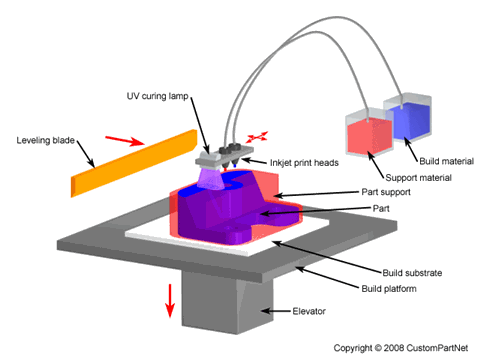
\includegraphics[width=0.6\textwidth]{SGC.png}
	\caption{Método SGC}
	\label{SGCdiagrama}
\end{figure}	

\end{frame}


\subsection{Modelado por deposición fundida [FDM]}

\begin{frame}
    
    \begin{block}{Modelado por deposición fundida [FDM]}
    	Usando filamentos previamente extruidos, el modelado por deposición fundida, usa una tobera para depositar material fundido sobre una estructura soporte, capa a capa.
    \end{block}

\begin{figure}[h!]
	\centering
	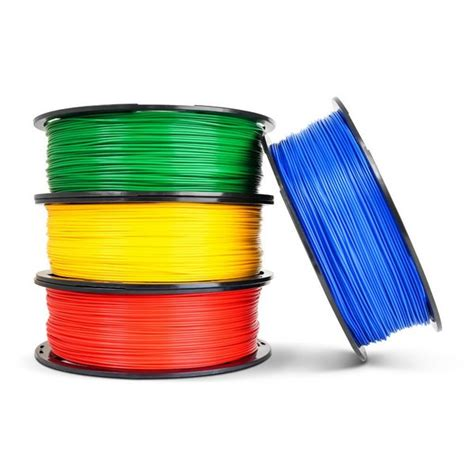
\includegraphics[width=0.4\textwidth]{PLA}
	\caption{Filamento previamete extruido}
	\label{Filamento}
\end{figure}
    
\end{frame}

\begin{frame}
%\frametitle{}
\begin{figure}[h!]
	\centering
	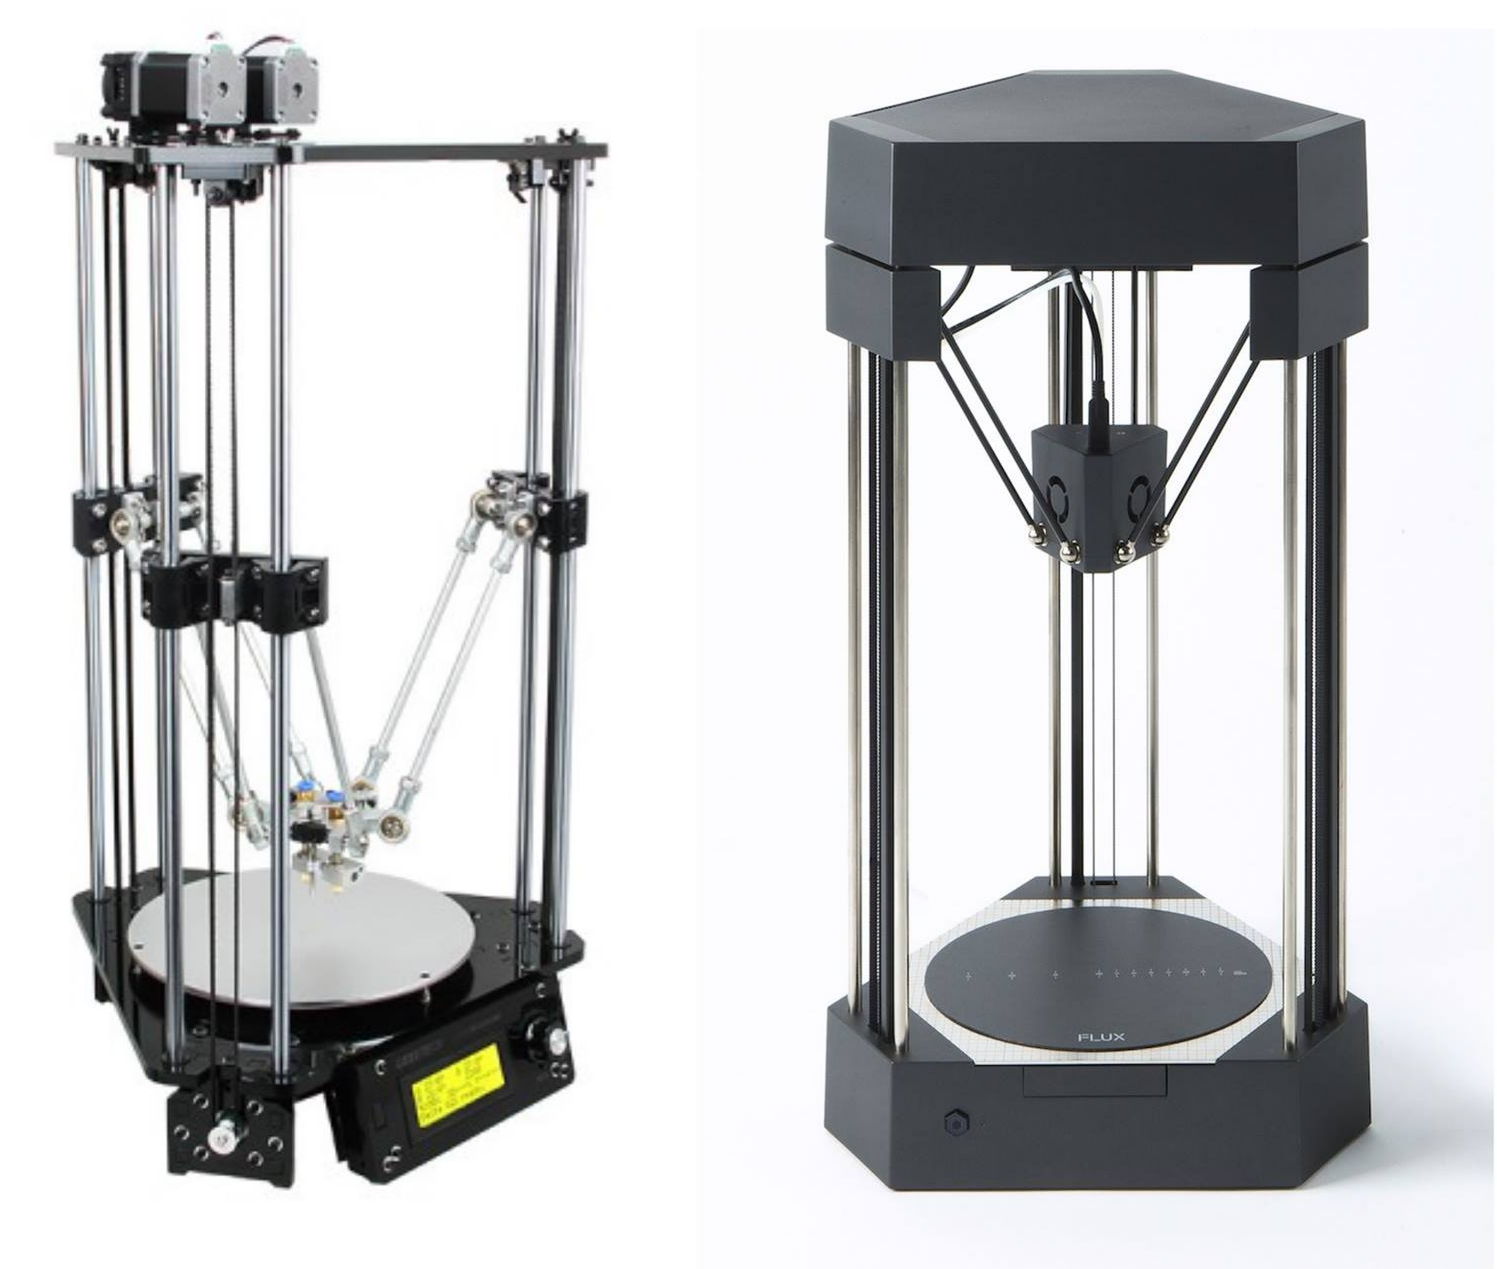
\includegraphics[width=0.6\textwidth]{maquinasFDM.png}
	\caption{Impresoras 3D tipo Delta}
	\label{Delta}
\end{figure}

\end{frame}
%------------------------------------------------

\section{Diseño y Fabricación}

\begin{frame}
\begin{figure}[h!]
	\centering
	
\includegraphics[width=0.6\textwidth]{3dprinting.png}
	\caption{Diagrama de pasos}
	\label{Proceso}
\end{figure}

\begin{block}{Pasos para obtener un modelo en 3D}
	
	\begin{itemize}
		\item Objeto 3D
		\item Esterolitografía [.STL]
		\item Código máquina a partir de esterolitografía
		\item Fabricación
	\end{itemize}
	
\end{block}


\end{frame}

%------------------------------------------------

\section{Internet}

\begin{frame}
      \begin{figure}[h!]
   	\centering
   	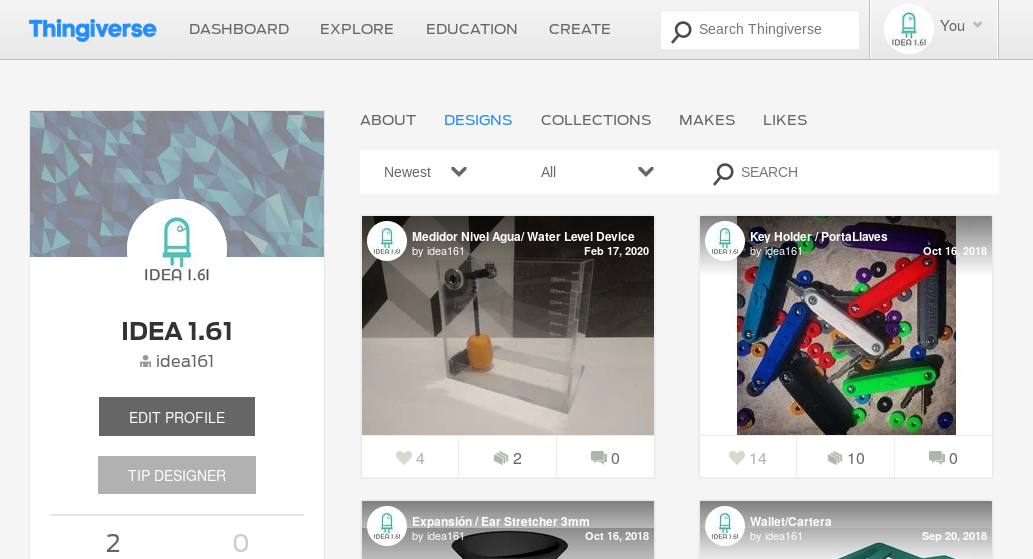
\includegraphics[width=0.8\textwidth]{thingiverse.png}
   	\caption{thingiverse.com/idea161/designs}
   	\label{thingiverse}
   \end{figure}
\end{frame}

\begin{frame}
\begin{figure}[h!]
	\centering
	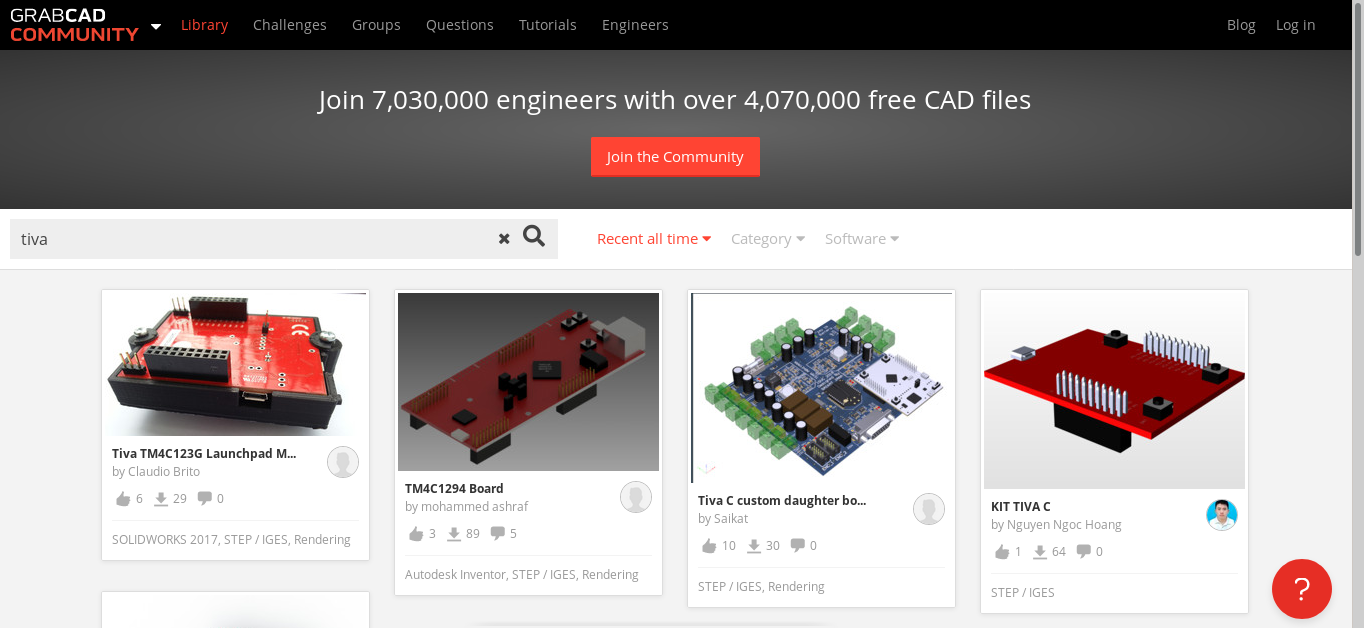
\includegraphics[width=0.8\textwidth]{grabcad.png}
	\caption{grabcad.com}
	\label{grabcad}
\end{figure}
\end{frame}

\section{Software}

\subsection{Software Diseño}

\begin{frame}
	
  \begin{block}{Diseño 3D Libres}
	\begin{itemize}
		\item OpenSCAD
		\item FreeCAD
		\item Blender
	\end{itemize}
  \end{block}

\begin{block}{Diseño 3D no libres}
	\begin{itemize}
		\item Fusion 360
		\item ThinkerCAD
		\item SOLIDWORKS
	\end{itemize}
\end{block}

%\begin{block}{Nota}
%	En algunos casos los programas se tiene más utilidades además del particionado como gestión de las características de la impresión en 3D, esto depende del firmware de cada impresora
%\end{block}
	
\end{frame}

%------------------------------------------------

\begin{frame}
   \begin{figure}[h!]
   	\centering
   	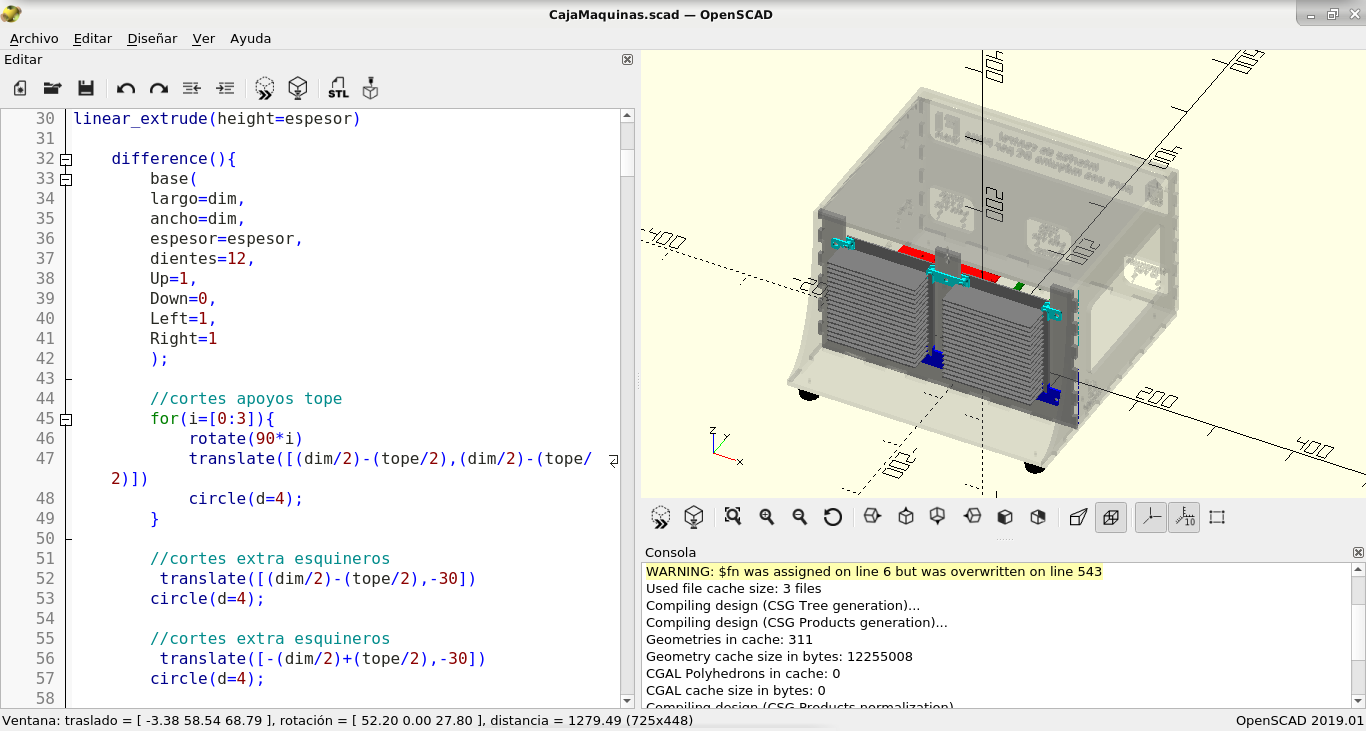
\includegraphics[width=0.8\textwidth]{OpenSCAD.png}
   	\caption{OpenSCAD}
   	\label{openscad}
   	\end{figure}
\end{frame}


%------------------------------------------------


\subsection{Software Particionado}

%------------------------------------------------

\begin{frame}

	
\begin{block}{Particionado}
	\begin{itemize}
		\item Slic3r
		\item Repetier
		\item Flux Studio
	\end{itemize}



\end{block}

\begin{figure}[h!]
	\centering
	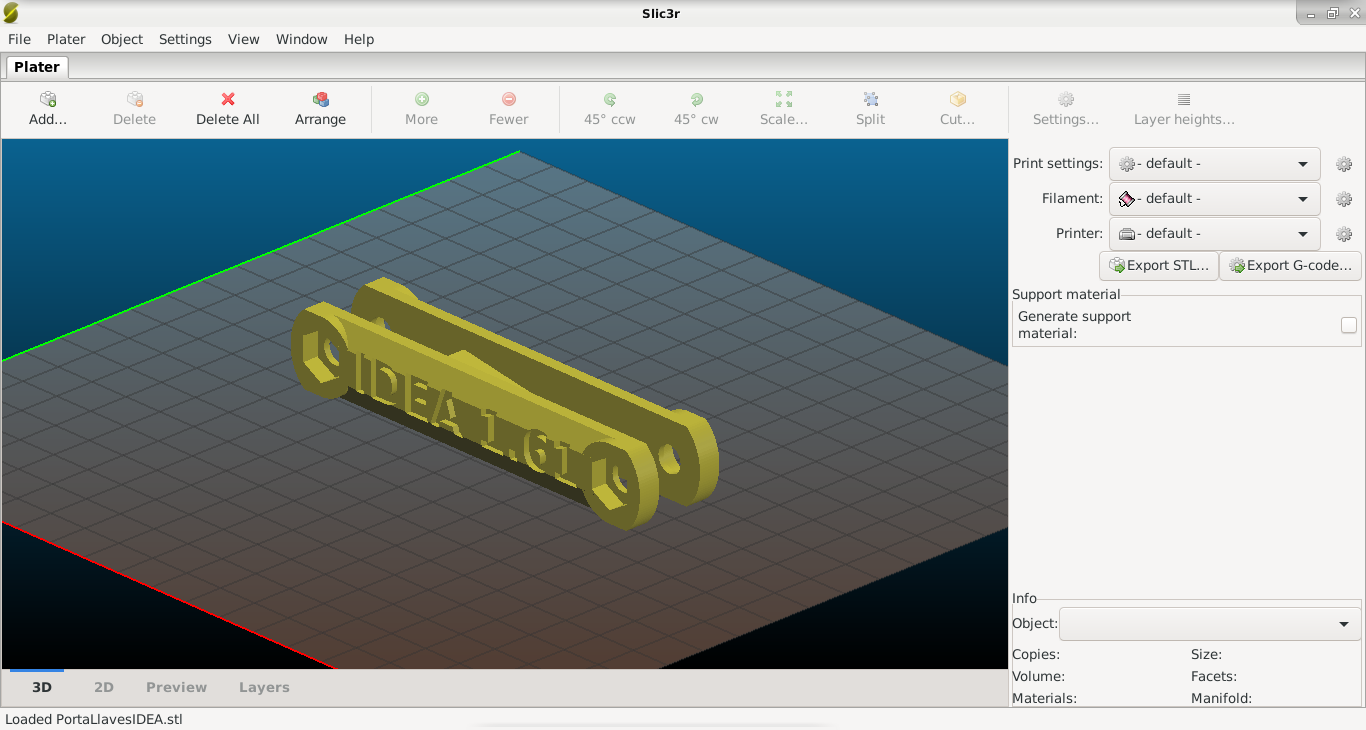
\includegraphics[width=0.6\textwidth]{slic3r.png}
	\caption{Slic3r}
	\label{slic3r}
\end{figure}   

   	
\end{frame}

%------------------------------------------------

\section{Aplicaciones}


\begin{frame}
      \begin{figure}[h!]
   	\centering
   	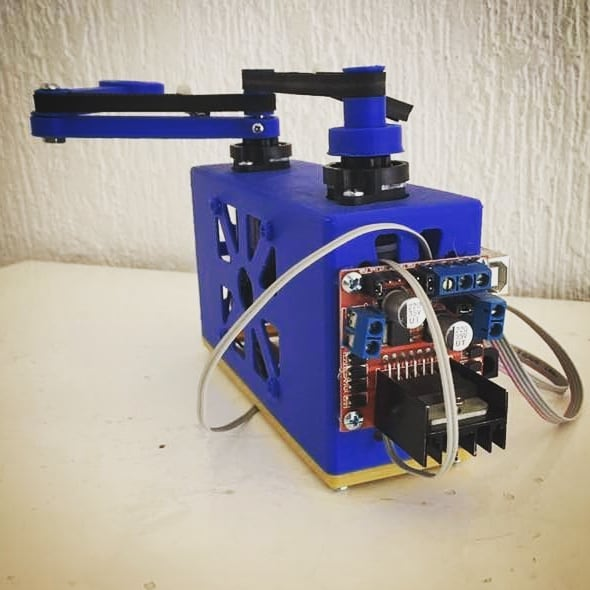
\includegraphics[width=0.6\textwidth]{BrazoAzul1}
   	\caption{Prototipos Electromecánicos}
   	\label{brazo}
   \end{figure}
\end{frame}

%-----

\begin{frame}
\begin{figure}[h!]
	\centering
	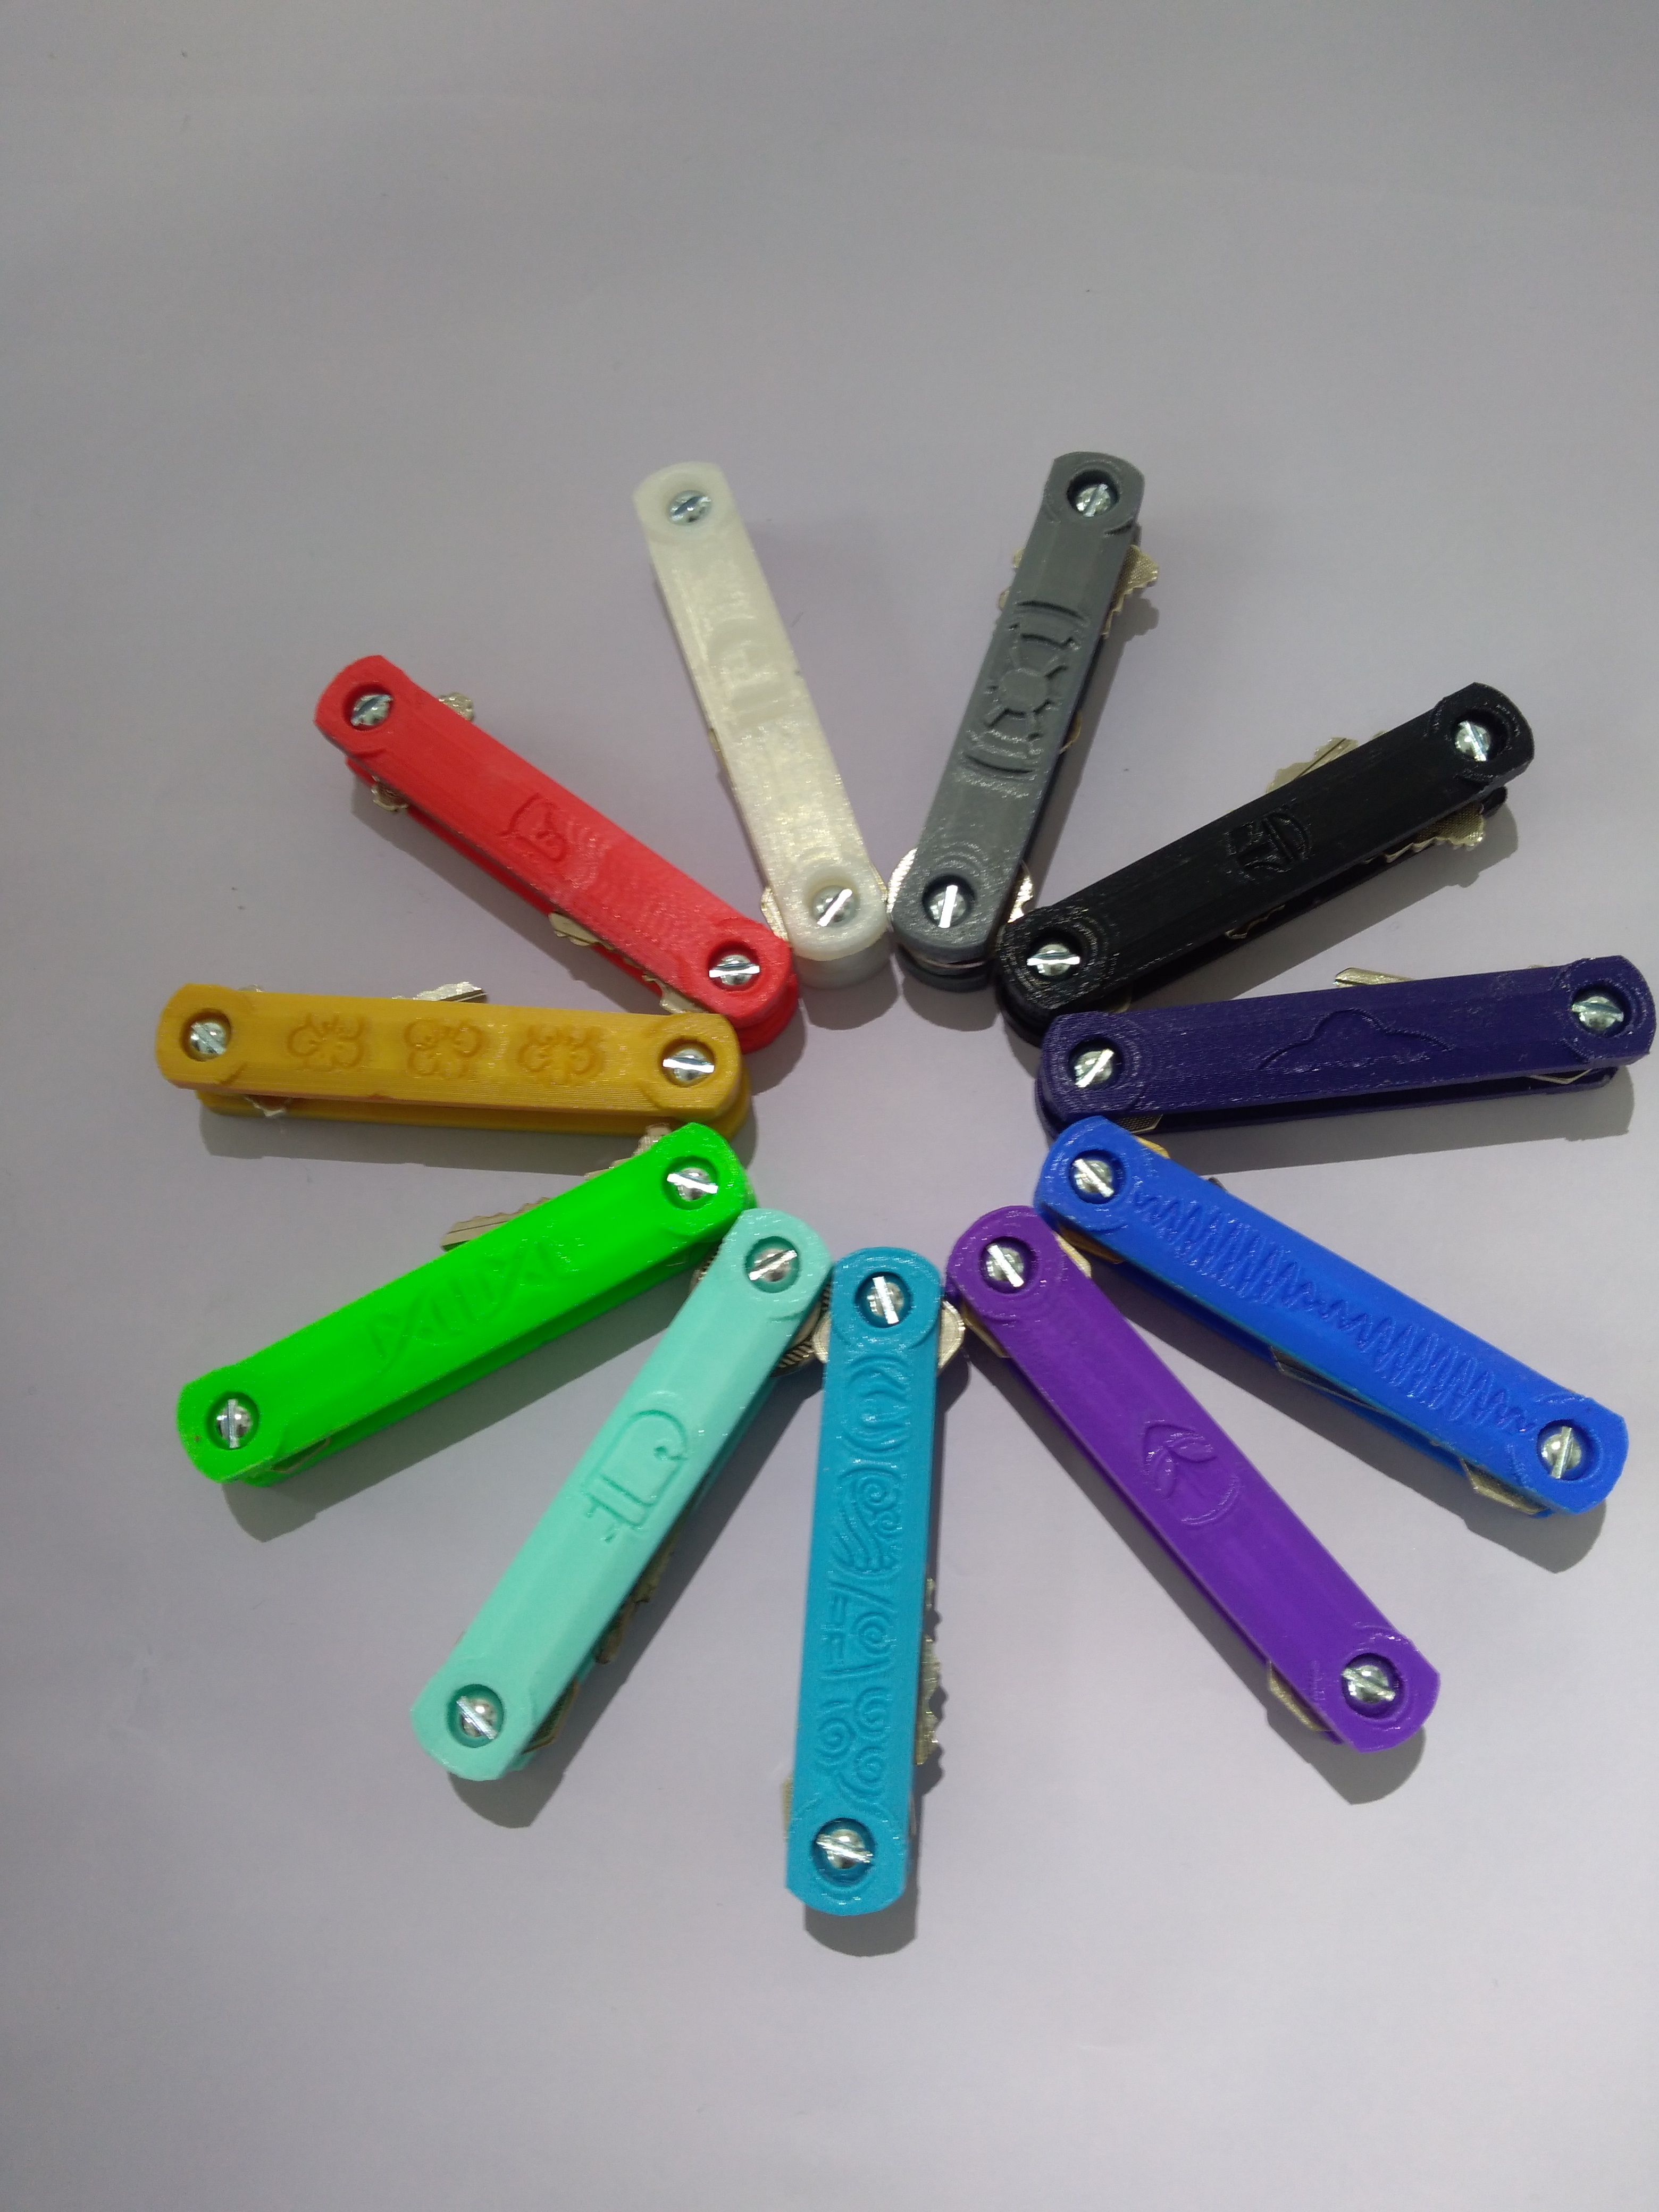
\includegraphics[width=0.4\textwidth]{portallaves}
	\caption{Objetos Utilitarios}
	\label{portallaves}
\end{figure}
\end{frame}

%------------------------------------------------


%\begin{frame}
%\frametitle{Referencias}

%\footnotesize{
%\begin{thebibliography}{99} % Beamer does not support BibTeX so references must be inserted manually as below
%\bibitem[Lamarsh2001]{p1} Lamarsh, John R and Baratta, Anthony J (2012)
%\newblock Introduction to Nuclear Engineering
%\newblock \emph{Third}. 

%\bibitem[InstitutoNacionalDeEstadisticayGeografia2018]{p2} INEGI (2018)
%\newblock cancer2018
%\newblock \emph{4 Febrero}.

%\bibitem[Niemantsverdriet2012]{p3} Niemantsverdriet (2012)
%\newblock High and low LET radiation differentially induce normal tissue damage signals
%\newblock \emph{2012}.
%\end{thebibliography}
%}
%\end{frame}

%------------------------------------------------

\begin{frame}
\Huge{\centerline{¡Gracias por su atención :D !}}
\end{frame}

%----------------------------------------------------------------------------------------

\end{document} 